\documentclass[conference,a4paper]{IEEEtran}
\IEEEoverridecommandlockouts
\usepackage[utf8]{inputenc}
\usepackage[T1]{fontenc}
\usepackage{amsmath,amssymb}
\usepackage{graphicx}
\usepackage{booktabs}
\usepackage{multirow}
\usepackage[table]{xcolor}
\usepackage{tikz}
\usetikzlibrary{arrows.meta,positioning,fit,calc,shapes.geometric}
\usepackage{cite}
\usepackage{xurl}
\usepackage[hidelinks]{hyperref}
\usepackage{balance}

% ---- Nombres en español (la instalación usada no incluye babel-spanish) ----
\renewcommand{\figurename}{Fig.}
\renewcommand{\tablename}{TABLA}
\renewcommand{\refname}{Referencias}
\renewcommand{\abstractname}{Resumen}
\def\IEEEkeywordsname{Palabras clave}
\renewcommand{\IEEEkeywordsname}{Palabras clave}
\makeatletter
\def\@IEEEabstractname{Resumen}
\makeatother

% Archivo generado automáticamente por src/macros_latex.py — no editar a mano
\newcommand{\accMN}{95{,}8}
\newcommand{\fMN}{95{,}7}
\newcommand{\eceRawMN}{10{,}6}
\newcommand{\eceCalMN}{1{,}5}
\newcommand{\nllRawMN}{0{,}200}
\newcommand{\nllCalMN}{0{,}104}
\newcommand{\TMN}{0{,}51}
\newcommand{\umbralMN}{60{,}6}
\newcommand{\cobMN}{97{,}2}
\newcommand{\rechMN}{2{,}8}
\newcommand{\accSelMN}{97{,}3}
\newcommand{\errAutoMN}{18}
\newcommand{\errRevMN}{11}
\newcommand{\okRevMN}{8}
\newcommand{\errTotMN}{29}
\newcommand{\latUnoMN}{13{,}5}
\newcommand{\latUnoPnMN}{17{,}2}
\newcommand{\latDosMN}{14{,}6}
\newcommand{\latDosPnMN}{19{,}4}
\newcommand{\latPreMN}{1{,}3}
\newcommand{\paramsMN}{4{,}21}
\newcommand{\gmacsMN}{0{,}22}
\newcommand{\tamMN}{17{,}0}
\newcommand{\epocaMN}{10}
\newcommand{\epocasMN}{11}
\newcommand{\minMN}{13}
\newcommand{\fValMN}{95{,}4}
\newcommand{\PPlaMN}{95{,}2}
\newcommand{\RPlaMN}{93{,}7}
\newcommand{\FPlaMN}{94{,}4}
\newcommand{\NPla}{127}
\newcommand{\PPapMN}{98{,}6}
\newcommand{\RPapMN}{96{,}7}
\newcommand{\FPapMN}{97{,}6}
\newcommand{\NPap}{150}
\newcommand{\PVidMN}{96{,}5}
\newcommand{\RVidMN}{92{,}0}
\newcommand{\FVidMN}{94{,}2}
\newcommand{\NVid}{150}
\newcommand{\PMetMN}{91{,}7}
\newcommand{\RMetMN}{97{,}4}
\newcommand{\FMetMN}{94{,}5}
\newcommand{\NMet}{114}
\newcommand{\POrgMN}{96{,}0}
\newcommand{\ROrgMN}{99{,}3}
\newcommand{\FOrgMN}{97{,}6}
\newcommand{\NOrg}{146}
\newcommand{\accFuenteGcMN}{97{,}5}
\newcommand{\nFuenteGc}{393}
\newcommand{\accFuenteTnMN}{93{,}5}
\newcommand{\nFuenteTn}{294}
\newcommand{\robOrigMN}{95{,}8}
\newcommand{\robRechOrigMN}{2{,}8}
\newcommand{\robSelOrigMN}{97{,}3}
\newcommand{\robOscuroMN}{95{,}3}
\newcommand{\robRechOscuroMN}{3{,}3}
\newcommand{\robSelOscuroMN}{96{,}8}
\newcommand{\robClaroMN}{92{,}9}
\newcommand{\robRechClaroMN}{2{,}8}
\newcommand{\robSelClaroMN}{94{,}0}
\newcommand{\robContrasteMN}{94{,}9}
\newcommand{\robRechContrasteMN}{3{,}8}
\newcommand{\robSelContrasteMN}{97{,}0}
\newcommand{\robBlurMN}{89{,}2}
\newcommand{\robRechBlurMN}{6{,}0}
\newcommand{\robSelBlurMN}{91{,}2}
\newcommand{\robRuidoMN}{91{,}8}
\newcommand{\robRechRuidoMN}{6{,}8}
\newcommand{\robSelRuidoMN}{95{,}2}
\newcommand{\robJpegMN}{93{,}2}
\newcommand{\robRechJpegMN}{4{,}7}
\newcommand{\robSelJpegMN}{95{,}3}
\newcommand{\robRotMN}{95{,}1}
\newcommand{\robRechRotMN}{3{,}3}
\newcommand{\robSelRotMN}{96{,}8}
\newcommand{\opAUmbralMN}{60{,}6}
\newcommand{\opACobMN}{97{,}2}
\newcommand{\opASelMN}{97{,}3}
\newcommand{\opAErrMN}{18}
\newcommand{\opARevMN}{19}
\newcommand{\opBUmbralMN}{79{,}1}
\newcommand{\opBCobMN}{93{,}9}
\newcommand{\opBSelMN}{98{,}6}
\newcommand{\opBErrMN}{9}
\newcommand{\opBRevMN}{42}
\newcommand{\opCUmbralMN}{88{,}8}
\newcommand{\opCCobMN}{91{,}3}
\newcommand{\opCSelMN}{99{,}5}
\newcommand{\opCErrMN}{3}
\newcommand{\opCRevMN}{60}
\newcommand{\nTest}{687}
\newcommand{\objetivoSel}{97}
\newcommand{\accEF}{96{,}8}
\newcommand{\fEF}{96{,}8}
\newcommand{\eceRawEF}{10{,}7}
\newcommand{\eceCalEF}{1{,}7}
\newcommand{\nllRawEF}{0{,}191}
\newcommand{\nllCalEF}{0{,}096}
\newcommand{\TEF}{0{,}55}
\newcommand{\umbralEF}{57{,}8}
\newcommand{\cobEF}{98{,}3}
\newcommand{\rechEF}{1{,}7}
\newcommand{\accSelEF}{97{,}6}
\newcommand{\errAutoEF}{16}
\newcommand{\errRevEF}{6}
\newcommand{\okRevEF}{6}
\newcommand{\errTotEF}{22}
\newcommand{\latUnoEF}{24{,}9}
\newcommand{\latUnoPnEF}{32{,}2}
\newcommand{\latDosEF}{21{,}4}
\newcommand{\latDosPnEF}{25{,}8}
\newcommand{\latPreEF}{1{,}1}
\newcommand{\paramsEF}{4{,}01}
\newcommand{\gmacsEF}{0{,}38}
\newcommand{\tamEF}{16{,}3}
\newcommand{\epocaEF}{8}
\newcommand{\epocasEF}{9}
\newcommand{\minEF}{28}
\newcommand{\fValEF}{96{,}1}
\newcommand{\PPlaEF}{96{,}1}
\newcommand{\RPlaEF}{96{,}9}
\newcommand{\FPlaEF}{96{,}5}
\newcommand{\PPapEF}{99{,}3}
\newcommand{\RPapEF}{96{,}0}
\newcommand{\FPapEF}{97{,}6}
\newcommand{\PVidEF}{97{,}3}
\newcommand{\RVidEF}{94{,}7}
\newcommand{\FVidEF}{95{,}9}
\newcommand{\PMetEF}{94{,}9}
\newcommand{\RMetEF}{97{,}4}
\newcommand{\FMetEF}{96{,}1}
\newcommand{\POrgEF}{96{,}0}
\newcommand{\ROrgEF}{99{,}3}
\newcommand{\FOrgEF}{97{,}6}
\newcommand{\accFuenteGcEF}{97{,}7}
\newcommand{\accFuenteTnEF}{95{,}6}
\newcommand{\robOrigEF}{96{,}8}
\newcommand{\robRechOrigEF}{1{,}7}
\newcommand{\robSelOrigEF}{97{,}6}
\newcommand{\robOscuroEF}{95{,}1}
\newcommand{\robRechOscuroEF}{2{,}8}
\newcommand{\robSelOscuroEF}{96{,}3}
\newcommand{\robClaroEF}{94{,}2}
\newcommand{\robRechClaroEF}{3{,}9}
\newcommand{\robSelClaroEF}{95{,}6}
\newcommand{\robContrasteEF}{95{,}6}
\newcommand{\robRechContrasteEF}{3{,}2}
\newcommand{\robSelContrasteEF}{96{,}7}
\newcommand{\robBlurEF}{89{,}1}
\newcommand{\robRechBlurEF}{8{,}7}
\newcommand{\robSelBlurEF}{92{,}3}
\newcommand{\robRuidoEF}{92{,}4}
\newcommand{\robRechRuidoEF}{3{,}2}
\newcommand{\robSelRuidoEF}{93{,}8}
\newcommand{\robJpegEF}{94{,}3}
\newcommand{\robRechJpegEF}{3{,}3}
\newcommand{\robSelJpegEF}{95{,}3}
\newcommand{\robRotEF}{95{,}9}
\newcommand{\robRechRotEF}{1{,}9}
\newcommand{\robSelRotEF}{96{,}4}
\newcommand{\opAUmbralEF}{57{,}8}
\newcommand{\opACobEF}{98{,}3}
\newcommand{\opASelEF}{97{,}6}
\newcommand{\opAErrEF}{16}
\newcommand{\opARevEF}{12}
\newcommand{\opBUmbralEF}{80{,}1}
\newcommand{\opBCobEF}{94{,}2}
\newcommand{\opBSelEF}{98{,}8}
\newcommand{\opBErrEF}{8}
\newcommand{\opBRevEF}{40}
\newcommand{\opCUmbralEF}{94{,}8}
\newcommand{\opCCobEF}{86{,}0}
\newcommand{\opCSelEF}{99{,}7}
\newcommand{\opCErrEF}{2}
\newcommand{\opCRevEF}{96}
\newcommand{\accRN}{96{,}4}
\newcommand{\fRN}{96{,}2}
\newcommand{\eceRawRN}{11{,}0}
\newcommand{\eceCalRN}{2{,}3}
\newcommand{\nllRawRN}{0{,}198}
\newcommand{\nllCalRN}{0{,}111}
\newcommand{\TRN}{0{,}55}
\newcommand{\umbralRN}{69{,}4}
\newcommand{\cobRN}{96{,}7}
\newcommand{\rechRN}{3{,}3}
\newcommand{\accSelRN}{97{,}7}
\newcommand{\errAutoRN}{15}
\newcommand{\errRevRN}{10}
\newcommand{\okRevRN}{13}
\newcommand{\errTotRN}{25}
\newcommand{\latUnoRN}{100{,}7}
\newcommand{\latUnoPnRN}{124{,}6}
\newcommand{\latDosRN}{63{,}4}
\newcommand{\latDosPnRN}{79{,}9}
\newcommand{\latPreRN}{1{,}2}
\newcommand{\paramsRN}{23{,}52}
\newcommand{\gmacsRN}{4{,}09}
\newcommand{\tamRN}{94{,}4}
\newcommand{\epocaRN}{8}
\newcommand{\epocasRN}{9}
\newcommand{\minRN}{54}
\newcommand{\fValRN}{95{,}2}
\newcommand{\PPlaRN}{94{,}4}
\newcommand{\RPlaRN}{93{,}7}
\newcommand{\FPlaRN}{94{,}1}
\newcommand{\PPapRN}{98{,}0}
\newcommand{\RPapRN}{97{,}3}
\newcommand{\FPapRN}{97{,}7}
\newcommand{\PVidRN}{97{,}3}
\newcommand{\RVidRN}{95{,}3}
\newcommand{\FVidRN}{96{,}3}
\newcommand{\PMetRN}{94{,}0}
\newcommand{\RMetRN}{95{,}6}
\newcommand{\FMetRN}{94{,}8}
\newcommand{\POrgRN}{97{,}3}
\newcommand{\ROrgRN}{99{,}3}
\newcommand{\FOrgRN}{98{,}3}
\newcommand{\accFuenteGcRN}{98{,}7}
\newcommand{\accFuenteTnRN}{93{,}2}
\newcommand{\robOrigRN}{96{,}4}
\newcommand{\robRechOrigRN}{3{,}3}
\newcommand{\robSelOrigRN}{97{,}7}
\newcommand{\robOscuroRN}{95{,}6}
\newcommand{\robRechOscuroRN}{4{,}1}
\newcommand{\robSelOscuroRN}{97{,}6}
\newcommand{\robClaroRN}{92{,}4}
\newcommand{\robRechClaroRN}{8{,}3}
\newcommand{\robSelClaroRN}{96{,}3}
\newcommand{\robContrasteRN}{95{,}8}
\newcommand{\robRechContrasteRN}{4{,}7}
\newcommand{\robSelContrasteRN}{97{,}9}
\newcommand{\robBlurRN}{89{,}5}
\newcommand{\robRechBlurRN}{14{,}7}
\newcommand{\robSelBlurRN}{93{,}9}
\newcommand{\robRuidoRN}{90{,}5}
\newcommand{\robRechRuidoRN}{10{,}5}
\newcommand{\robSelRuidoRN}{94{,}8}
\newcommand{\robJpegRN}{92{,}7}
\newcommand{\robRechJpegRN}{7{,}0}
\newcommand{\robSelJpegRN}{96{,}1}
\newcommand{\robRotRN}{94{,}8}
\newcommand{\robRechRotRN}{3{,}9}
\newcommand{\robSelRotRN}{97{,}1}
\newcommand{\opAUmbralRN}{69{,}4}
\newcommand{\opACobRN}{96{,}7}
\newcommand{\opASelRN}{97{,}7}
\newcommand{\opAErrRN}{15}
\newcommand{\opARevRN}{23}
\newcommand{\opBUmbralRN}{78{,}7}
\newcommand{\opBCobRN}{94{,}2}
\newcommand{\opBSelRN}{98{,}8}
\newcommand{\opBErrRN}{8}
\newcommand{\opBRevRN}{40}
\newcommand{\opCUmbralRN}{87{,}0}
\newcommand{\opCCobRN}{90{,}5}
\newcommand{\opCSelRN}{98{,}9}
\newcommand{\opCErrRN}{7}
\newcommand{\opCRevRN}{65}
\newcommand{\icAccMN}{94{,}3--97{,}2}
\newcommand{\icFMN}{94{,}1--97{,}1}
\newcommand{\icAccEF}{95{,}3--98{,}0}
\newcommand{\icFEF}{95{,}4--98{,}0}
\newcommand{\icAccRN}{94{,}9--97{,}7}
\newcommand{\icFRN}{94{,}7--97{,}6}
\newcommand{\mcnMNEF}{0{,}26}
\newcommand{\mcnBMNEF}{11}
\newcommand{\mcnCMNEF}{18}
\newcommand{\mcnMNRN}{0{,}63}
\newcommand{\mcnBMNRN}{17}
\newcommand{\mcnCMNRN}{21}
\newcommand{\mcnEFRN}{0{,}69}
\newcommand{\mcnBEFRN}{14}
\newcommand{\mcnCEFRN}{11}
\newcommand{\nTrainPla}{601}
\newcommand{\nTrainPap}{700}
\newcommand{\nTrainVid}{700}
\newcommand{\nTrainMet}{529}
\newcommand{\nTrainOrg}{683}
\newcommand{\nTrain}{3213}
\newcommand{\nValPla}{127}
\newcommand{\nValPap}{150}
\newcommand{\nValVid}{150}
\newcommand{\nValMet}{113}
\newcommand{\nValOrg}{147}
\newcommand{\nVal}{687}
\newcommand{\nTestPla}{127}
\newcommand{\nTestPap}{150}
\newcommand{\nTestVid}{150}
\newcommand{\nTestMet}{114}
\newcommand{\nTestOrg}{146}
\newcommand{\tnPla}{478}
\newcommand{\gcPla}{377}
\newcommand{\totPla}{855}
\newcommand{\tnPap}{500}
\newcommand{\gcPap}{500}
\newcommand{\totPap}{1000}
\newcommand{\tnVid}{497}
\newcommand{\gcVid}{503}
\newcommand{\totVid}{1000}
\newcommand{\tnMet}{405}
\newcommand{\gcMet}{351}
\newcommand{\totMet}{756}
\newcommand{\tnOrg}{0}
\newcommand{\gcOrg}{976}
\newcommand{\totOrg}{976}
\newcommand{\nTotal}{4587}
\newcommand{\nTotalTn}{1880}
\newcommand{\nTotalGc}{2707}


% ==================== Enlaces de la entrega (reemplazar) ====================
\newcommand{\linkGithub}{\url{https://github.com/josemo2921-creator/reciclia-clasificador-residuos}}
\newcommand{\linkDrive}{\url{https://drive.google.com/file/d/1hDcWeyB43BreaZ5l-OtWcR34YWTTz_ie/view?usp=sharing}}
\newcommand{\linkVideo}{\url{https://youtu.be/MqwA1bZAXf4}}
% ============================================================================

\begin{document}

\title{Clasificación automática de residuos reciclables en el punto de depósito con MobileNetV3 y rechazo calibrado de casos inciertos}

\author{
\IEEEauthorblockN{José David Moreno Ahumada}
\IEEEauthorblockA{Programa de Ingeniería de Sistemas\\
Universidad de Ibagué, Ibagué, Colombia\\
\texttt{jose.moreno@estudiantesunibague.edu.co}}
\and
\IEEEauthorblockN{Alexandra La Cruz}
\IEEEauthorblockA{Programa de Ingeniería de Sistemas\\
Universidad de Ibagué, Ibagué, Colombia\\
\texttt{alexandra.lacruz@unibague.edu.co}}
}

\maketitle

\begin{abstract}
La separación incorrecta de residuos en la fuente contamina lotes completos de material reciclable. Este trabajo presenta ReciclIA, un agente inteligente que observa un residuo mediante una cámara, lo asigna a una de cinco categorías (plástico, papel/cartón, vidrio, metal y orgánico), indica el contenedor según el código de colores colombiano y se abstiene de decidir cuando su confianza es baja. Se construyó un conjunto de \nTotal{} imágenes combinando TrashNet y Garbage Classification, con deduplicación perceptual que eliminó más de 2\,400 copias compartidas entre ambas fuentes y que habrían filtrado información entre entrenamiento y prueba. Se comparan MobileNetV3-Large, EfficientNet-B0 y ResNet-50 ajustados por aprendizaje por transferencia en dos fases. MobileNetV3 obtiene una exactitud de \accMN\,\% y un F1 macro de \fMN\,\% en un conjunto de prueba independiente de \nTest{} imágenes, con una latencia de \latUnoMN~ms por imagen en un solo núcleo de CPU. La calibración por escalamiento de temperatura reduce el error de calibración esperado de \eceRawMN\,\% a \eceCalMN\,\%, y un umbral de confianza elegido en validación eleva la exactitud de las decisiones automáticas a \accSelMN\,\%, enviando a revisión manual el \rechMN\,\% de los objetos. Se evalúa además la robustez ante cambios de iluminación, desenfoque, ruido y compresión, y se publica el código, el conjunto de datos procesado y una demostración web.
\end{abstract}

\begin{IEEEkeywords}
agentes inteligentes, clasificación de residuos, aprendizaje por transferencia, MobileNetV3, calibración, clasificación selectiva, visión por computadora.
\end{IEEEkeywords}

% =====================================================================
\section{Introducción}
% =====================================================================
Colombia aprovecha apenas el 16,9\,\% de sus residuos sólidos ordinarios \cite{dnp2025}. Una parte del problema ocurre en el primer eslabón de la cadena: el ciudadano frente al contenedor. Desde 2021 el país usa un código de colores unificado (blanco para aprovechables como plástico, vidrio, metal, papel y cartón; verde para orgánicos aprovechables; negro para no aprovechables) \cite{res2184}, pero elegir el contenedor correcto sigue dependiendo de que cada persona reconozca el material. Un solo objeto mal ubicado puede contaminar un lote de reciclaje completo.

Este artículo aborda esa decisión con un agente racional en el sentido de Russell y Norvig \cite{russell2021}: percibe el residuo mediante una cámara fija en una estación de reciclaje (universidad, oficina o vivienda), decide su categoría y actúa mostrando el resultado, señalando el contenedor y registrando el evento. A diferencia de un clasificador convencional, el agente tiene una cuarta acción disponible: declarar el residuo como \emph{incierto} y solicitar revisión manual cuando su confianza calibrada no alcanza un umbral. Esta opción responde a uno de los vacíos identificados en la revisión de la literatura del proyecto: la mayoría de los trabajos fuerzan una clase incluso ante objetos ambiguos, como envases con restos de comida.

Las contribuciones del trabajo son:
\begin{enumerate}
\item Un conjunto de datos de cinco clases que incluye la clase orgánica, construido a partir de dos fuentes públicas con deduplicación perceptual y partición sin fuga de información. Se documenta que la mayor parte de las imágenes de TrashNet aparecen también dentro de Garbage Classification, un solapamiento que infla los resultados si las fuentes se combinan sin depurar.
\item Una comparación controlada de tres arquitecturas preentrenadas (MobileNetV3-Large, EfficientNet-B0 y ResNet-50) que reporta conjuntamente exactitud, costo computacional y latencia en CPU.
\item Un mecanismo de rechazo basado en probabilidades calibradas, con su análisis de riesgo y cobertura, y una evaluación de robustez ante perturbaciones de captura.
\item Una implementación abierta del agente con demostración web.
\end{enumerate}

El resto del artículo se organiza así: la Sección~\ref{sec:relacionados} resume el estado del arte; la Sección~\ref{sec:metodos} describe el agente, los datos y los métodos; la Sección~\ref{sec:resultados} presenta y discute los resultados, y la Sección~\ref{sec:conclusiones} concluye.

% =====================================================================
\section{Trabajos relacionados}\label{sec:relacionados}
% =====================================================================
\textbf{Conjuntos de datos.} TrashNet \cite{trashnet} reúne 2\,527 fotografías en seis clases sobre fondo blanco uniforme y carece de clase orgánica. TACO \cite{taco} anota residuos en escenas naturales para detección, con fuerte desbalance. Garbage Classification \cite{gc12} agrupa 15\,150 imágenes web en doce clases, entre ellas una clase \emph{biological} de restos de comida y vegetales, y es una de las pocas fuentes públicas que cubre residuos orgánicos junto a los materiales reciclables.

\textbf{Clasificación con redes convolucionales.} Las arquitecturas VGG \cite{vgg}, ResNet \cite{resnet} y DenseNet \cite{densenet} dominaron la clasificación de imágenes. En residuos, SpotGarbage \cite{spotgarbage} detectó basura desde un teléfono móvil sin distinguir el material; Yang y Thung \cite{trashnet} observaron que un SVM con SIFT superaba a una CNN entrenada desde cero en TrashNet, por la escasez de datos. Trabajos posteriores mejoraron esos resultados con modelos híbridos \cite{chu2018}, características de ResNet-50 con SVM \cite{adedeji2019}, variantes de DenseNet \cite{recyclenet} y comparaciones de redes preentrenadas \cite{ruiz2019}. Zhang et~al. \cite{zhang2021} confirmaron que el aprendizaje por transferencia \cite{pan2010} supera al entrenamiento desde cero cuando los datos son limitados.

\textbf{Modelos ligeros y detección.} MobileNet \cite{mobilenet,mobilenetv2,mobilenetv3} y EfficientNet \cite{efficientnet} reducen el costo de inferencia para dispositivos de borde. Los detectores Faster R-CNN \cite{fasterrcnn}, SSD \cite{ssd} y YOLO \cite{yolo,yolov7} localizan varios objetos a la vez, a cambio de anotaciones más costosas. Los Vision Transformers \cite{vit,swin} y los modelos fundacionales como CLIP \cite{clip} prometen mejor generalización, con mayor costo computacional.

\textbf{Confiabilidad.} El aumento de datos \cite{shorten2019} simula variaciones de captura; las redes modernas tienden a ser sobreconfiadas y el escalamiento de temperatura corrige esa tendencia con un solo parámetro \cite{guo2017}; la clasificación selectiva formaliza la opción de abstenerse para garantizar un nivel de riesgo \cite{geifman2017}; la robustez ante corrupciones comunes se mide perturbando sistemáticamente el conjunto de prueba \cite{hendrycks2019}, y Grad-CAM \cite{gradcam} muestra en qué regiones se apoya la decisión.

\textbf{Vacíos.} La revisión muestra resultados evaluados mayoritariamente en fondos uniformes, escasa medición de latencia en hardware modesto, poca atención a la abstención ante objetos ambiguos y cobertura limitada de la clase orgánica. Este trabajo atiende esos cuatro puntos.

% =====================================================================
\section{Métodos}\label{sec:metodos}
% =====================================================================
\subsection{Formulación como agente}
La Tabla~\ref{tab:peas} resume el agente con el esquema PEAS (medida de desempeño, entorno, actuadores y sensores) \cite{russell2021}, y la Fig.~\ref{fig:agente} muestra su ciclo de percepción, decisión y acción. El entorno es parcialmente observable (una sola vista del objeto), episódico (cada residuo es independiente), estático durante la decisión y discreto en sus acciones.

\begin{table}[t]
\caption{Descripción PEAS del agente ReciclIA}\label{tab:peas}
\centering\footnotesize
\begin{tabular}{@{}p{0.23\columnwidth}p{0.70\columnwidth}@{}}
\toprule
Desempeño & Exactitud y F1 por clase; exactitud de las decisiones automáticas; tasa de rechazo; latencia por imagen. \\
Entorno & Estación de reciclaje con cámara fija; un residuo por vez; iluminación y fondo variables. \\
Actuadores & Pantalla con la categoría y el contenedor; señal visual; solicitud de revisión manual; registro CSV de eventos. \\
Sensores & Cámara RGB (fotografía o cuadro de video). \\
\bottomrule
\end{tabular}
\end{table}

\begin{figure*}[t]
\centering
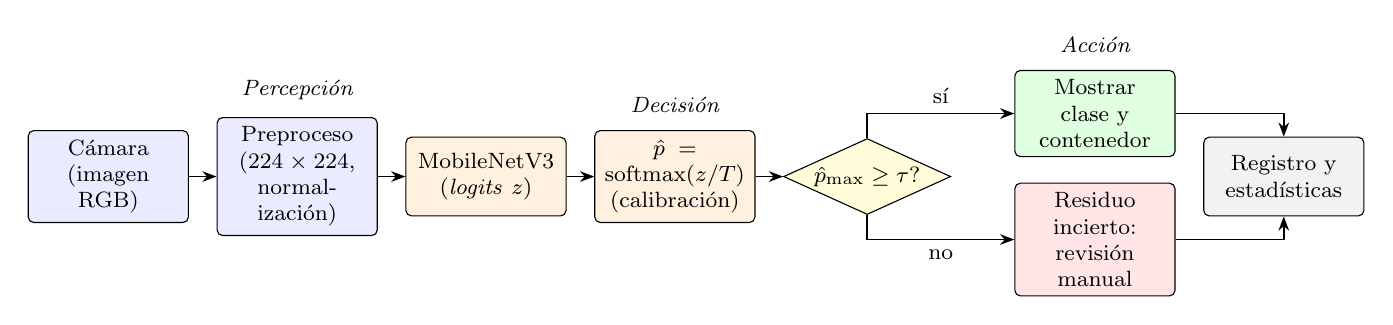
\begin{tikzpicture}[
  font=\footnotesize, node distance=3.5mm,
  caja/.style={draw, rounded corners=2pt, align=center, minimum height=10mm, text width=18mm, fill=#1},
  caja/.default=white, flecha/.style={-{Stealth[length=1.8mm]}, semithick}]
\node[caja=blue!8] (cam) {Cámara\\(imagen RGB)};
\node[caja=blue!8, right=of cam] (pre) {Preproceso\\($224\times224$, normalización)};
\node[caja=orange!12, right=of pre] (cnn) {MobileNetV3\\(\emph{logits} $z$)};
\node[caja=orange!12, right=of cnn] (cal) {$\hat p=\mathrm{softmax}(z/T)$\\(calibración)};
\node[draw, diamond, aspect=2.2, inner sep=1pt, align=center, fill=yellow!15, right=of cal] (dec) {$\hat p_{\max}\geq\tau$?};
\node[caja=green!12, right=8mm of dec, yshift=8mm] (ok) {Mostrar clase y\\contenedor};
\node[caja=red!10, right=8mm of dec, yshift=-8mm] (rev) {Residuo incierto:\\revisión manual};
\node[caja=gray!10, right=of ok, yshift=-8mm] (log) {Registro y\\estadísticas};
\draw[flecha] (cam) -- (pre); \draw[flecha] (pre) -- (cnn); \draw[flecha] (cnn) -- (cal); \draw[flecha] (cal) -- (dec);
\draw[flecha] (dec.north) |- node[above, pos=0.75]{sí} (ok.west);
\draw[flecha] (dec.south) |- node[below, pos=0.75]{no} (rev.west);
\draw[flecha] (ok.east) -| (log.north); \draw[flecha] (rev.east) -| (log.south);
\node[above=1mm of pre, font=\footnotesize\itshape] {Percepción};
\node[above=1mm of cal, font=\footnotesize\itshape] {Decisión};
\node[above=1mm of ok, font=\footnotesize\itshape] {Acción};
\end{tikzpicture}
\caption{Ciclo del agente. La acción depende de la confianza calibrada $\hat p_{\max}$: si alcanza el umbral $\tau$ se informa la categoría y el contenedor; si no, se solicita revisión manual. Todas las decisiones se registran.}
\label{fig:agente}
\end{figure*}

\subsection{Conjunto de datos}
Se combinaron dos fuentes públicas. De TrashNet \cite{trashnet} se tomaron las clases \emph{plastic}, \emph{paper}, \emph{cardboard}, \emph{glass} y \emph{metal}, y se descartó \emph{trash} por mezclar materiales. De Garbage Classification \cite{gc12}, obtenido de una réplica pública en GitHub, se tomaron \emph{plastic}, \emph{paper}, \emph{cardboard}, \emph{metal}, las tres clases de vidrio (\emph{brown}, \emph{green} y \emph{white-glass}) y \emph{biological}. Las etiquetas se mapearon a las cinco clases del proyecto: papel y cartón se fusionan, las tres clases de vidrio se fusionan y \emph{biological} pasa a ser orgánico. En total se listaron 8\,961 imágenes.

\textbf{Deduplicación.} Se calculó el \emph{hash} perceptual (pHash) \cite{zauner2010} de cada imagen y se agruparon las parejas con distancia de Hamming $\leq 4$ bits. Se hallaron 2\,417 parejas de casi-duplicados entre fuentes distintas, 2\,415 de ellas idénticas: casi todo TrashNet está contenido en Garbage Classification. Se eliminaron 2\,451 copias y 32 imágenes cuyos duplicados tenían etiquetas contradictorias, quedando 6\,478 imágenes únicas. Sin este paso, una misma fotografía podría quedar a la vez en entrenamiento y prueba.

\textbf{Balance y partición.} Para equilibrar clases y fondos se tomaron por clase hasta 500 imágenes de TrashNet (fondo uniforme) y se completó hasta 1\,000 con Garbage Classification (fondos variados). El resultado son \nTotal{} imágenes (Fig.~\ref{fig:dataset} y Tabla~\ref{tab:datos}); la Fig.~\ref{fig:ejemplos} muestra ejemplos de cada fuente. La clase orgánica proviene únicamente de Garbage Classification, lo que se analiza como limitación en la Sección~\ref{sec:discusion}. La partición se hizo de forma estratificada en proporción 70/15/15 (semilla 42) después de colapsar los duplicados, de modo que ninguna imagen ni sus copias aparecen en más de un subconjunto. Las imágenes se almacenaron con el lado mayor reducido a 384 píxeles.

\begin{figure}[t]
\centering
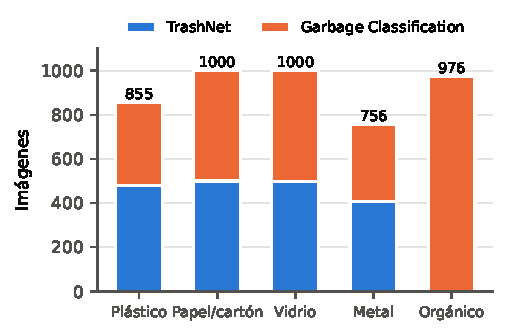
\includegraphics[width=\columnwidth]{figuras/fig_dataset.pdf}
\caption{Composición del conjunto de datos final por clase y por fuente.}
\label{fig:dataset}
\end{figure}

\begin{table}[t]
\caption{Imágenes por clase, fuente y partición}\label{tab:datos}
\centering\footnotesize\setlength{\tabcolsep}{3pt}
\begin{tabular}{@{}lrrrrrr@{}}
\toprule
Clase & TrashNet & Garbage C. & Entren. & Valid. & Prueba & Total \\
\midrule
Plástico & \tnPla & \gcPla & \nTrainPla & \nValPla & \nTestPla & \totPla \\
Papel/cartón & \tnPap & \gcPap & \nTrainPap & \nValPap & \nTestPap & \totPap \\
Vidrio & \tnVid & \gcVid & \nTrainVid & \nValVid & \nTestVid & \totVid \\
Metal & \tnMet & \gcMet & \nTrainMet & \nValMet & \nTestMet & \totMet \\
Orgánico & \tnOrg & \gcOrg & \nTrainOrg & \nValOrg & \nTestOrg & \totOrg \\
\midrule
Total & \nTotalTn & \nTotalGc & \nTrain & \nVal & \nTest & \nTotal \\
\bottomrule
\end{tabular}
\end{table}

\begin{figure*}[t]
\centering
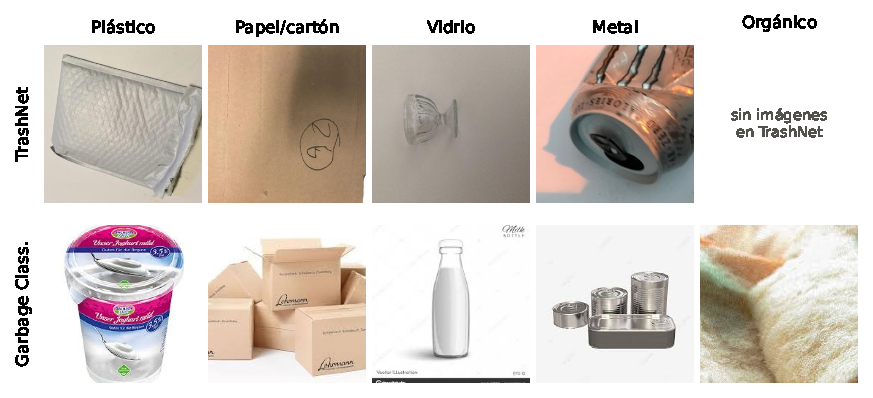
\includegraphics[width=0.85\textwidth]{figuras/fig_ejemplos.pdf}
\caption{Ejemplos del conjunto de entrenamiento. Fila superior: TrashNet (fondo blanco uniforme). Fila inferior: Garbage Classification (fondos e iluminación variados). TrashNet no contiene residuos orgánicos.}
\label{fig:ejemplos}
\end{figure*}

\subsection{Modelos y entrenamiento}
Se compararon tres redes preentrenadas en ImageNet \cite{imagenet}, tomadas de la biblioteca \texttt{timm} \cite{timm} sobre PyTorch \cite{pytorch}: MobileNetV3-Large \cite{mobilenetv3}, el modelo base propuesto en las fases anteriores por su bajo costo; EfficientNet-B0 \cite{efficientnet}, y ResNet-50 \cite{resnet} como referencia de mayor capacidad. En cada una se reemplazó la capa de clasificación por una de cinco salidas.

El ajuste se hizo en dos fases. En la fase~1 (3 épocas) se congeló la red y se entrenó solo la cabeza con tasa de aprendizaje $3\times10^{-3}$. En la fase~2 se descongelaron las dos últimas etapas convolucionales y la cabeza (la etapa \texttt{layer4} en ResNet-50) con tasa $5\times10^{-4}$ y decaimiento coseno; MobileNetV3 se ajustó durante 8 épocas en esta fase y los otros dos modelos durante 6. Las capas de normalización por lotes congeladas se mantuvieron en modo de inferencia. Se usó AdamW \cite{adamw} con decaimiento de pesos $10^{-4}$, entropía cruzada con suavizado de etiquetas de 0,1 \cite{szegedy2016}, lotes de 32 imágenes de $224\times224$ y aumento de datos \cite{shorten2019} con recorte aleatorio (escala 0,6--1), volteo horizontal, rotación de $\pm15^\circ$ y variación de brillo, contraste, saturación y tono. Se conservó el modelo de la época con mayor F1 macro en validación. Todo el entrenamiento se ejecutó en CPU (2 núcleos Intel Xeon a 2,1~GHz), sin GPU, con semilla fija (42).

\subsection{Calibración y rechazo}
Sea $z$ el vector de \emph{logits}. El escalamiento de temperatura \cite{guo2017} produce probabilidades $\hat p = \mathrm{softmax}(z/T)$, donde el escalar $T>0$ se ajusta minimizando la log-verosimilitud negativa en validación; no cambia la clase predicha, solo la confianza. La calidad de la calibración se mide con el error de calibración esperado \cite{naeini2015},
\begin{equation}
\mathrm{ECE}=\sum_{b=1}^{B}\frac{|S_b|}{n}\,\bigl|\mathrm{acc}(S_b)-\mathrm{conf}(S_b)\bigr|,
\end{equation}
con $B=15$ intervalos de confianza $S_b$. El agente clasifica automáticamente solo si $\hat p_{\max}\geq\tau$ \cite{geifman2017}. El umbral $\tau$ se eligió en validación como el menor valor cuya exactitud sobre las imágenes aceptadas alcanza el \objetivoSel\,\%; así se maximiza la cobertura (fracción de imágenes decididas sin intervención) sujeta a ese nivel de riesgo. El umbral se aplica sin modificaciones al conjunto de prueba.

\subsection{Protocolo de evaluación}
Sobre el conjunto de prueba (\nTest{} imágenes nunca usadas para entrenar ni para elegir hiperparámetros) se reportan exactitud, precisión, exhaustividad (\emph{recall}) y F1 por clase, F1 macro, matriz de confusión, ECE, cobertura y exactitud selectiva. Para medir robustez ante condiciones de captura \cite{hendrycks2019} se repitió la evaluación aplicando siete perturbaciones a todas las imágenes de prueba: baja iluminación (brillo $\times0{,}45$), sobreexposición ($\times1{,}7$), bajo contraste ($\times0{,}45$), desenfoque gaussiano (radio 2,5), ruido gaussiano ($\sigma=0{,}08$), compresión JPEG (calidad 15) y rotación de $30^\circ$. La latencia se midió como el promedio de 100 inferencias con una imagen, tras 10 de calentamiento, con 1 y 2 hilos de CPU. Grad-CAM \cite{gradcam} se aplicó sobre el último mapa de características para inspeccionar aciertos y errores.

\subsection{Implementación}
El agente se implementó en Python como una clase con los métodos \texttt{percibir}, \texttt{decidir} y \texttt{actuar}; la acción asocia cada clase al contenedor de la Resolución 2184 de 2019 \cite{res2184} (blanco para plástico, papel/cartón, vidrio y metal; verde para orgánico) y escribe cada evento en un registro CSV del que se obtienen estadísticas de uso. La demostración web usa Gradio \cite{gradio} y acepta una fotografía o la cámara del equipo. El código está disponible en \linkGithub.

% =====================================================================
\section{Resultados y discusión}\label{sec:resultados}
% =====================================================================
\subsection{Comparación de arquitecturas}
La Tabla~\ref{tab:modelos} compara los tres modelos en el conjunto de prueba, y la Fig.~\ref{fig:curvas} muestra la evolución del F1 macro en validación. Los tres modelos quedan a menos de un punto porcentual de exactitud entre sí (MobileNetV3 \accMN\,\%, EfficientNet-B0 \accEF\,\% y ResNet-50 \accRN\,\%), sus intervalos de confianza se solapan y la prueba de McNemar sobre las predicciones pareadas no encuentra diferencias significativas en ningún par ($p=\mcnMNEF$ para MobileNetV3 frente a EfficientNet-B0, $p=\mcnMNRN$ frente a ResNet-50 y $p=\mcnEFRN$ entre estos dos). Las diferencias sí son grandes en costo: ResNet-50 tiene unas 5,6 veces más parámetros y unas 19 veces más operaciones que MobileNetV3, y es unas 7 veces más lenta con un hilo (\latUnoRN{} frente a \latUnoMN~ms); EfficientNet-B0 tiene un tamaño similar al de MobileNetV3, pero casi el doble de operaciones y una latencia de \latUnoEF~ms. Con una exactitud estadísticamente equivalente y el menor costo de inferencia, se selecciona MobileNetV3 como modelo del agente; el resto de la sección se centra en él, salvo donde se comparan los tres.

\begin{table*}[t]
\caption{Comparación de modelos en el conjunto de prueba (\nTest{} imágenes). Intervalos de confianza del 95\,\% por \emph{bootstrap} (2\,000 remuestreos). Latencia: promedio de una inferencia con una imagen de $224\times224$ en CPU (Intel Xeon 2,1~GHz)}
\label{tab:modelos}
\centering\footnotesize
\begin{tabular}{@{}lrrrcccrr@{}}
\toprule
Modelo & Parám. (M) & GMACs & MB & Exactitud (\%) [IC 95\,\%] & F1 macro (\%) & ECE cal. (\%) & Lat. 1 hilo (ms) & Lat. 2 hilos (ms) \\
\midrule
MobileNetV3-Large & \paramsMN & \gmacsMN & \tamMN & \accMN{} [\icAccMN] & \fMN & \eceCalMN & \textbf{\latUnoMN} & \textbf{\latDosMN} \\
EfficientNet-B0 & \paramsEF & \gmacsEF & \tamEF & \accEF{} [\icAccEF] & \fEF & \eceCalEF & \latUnoEF & \latDosEF \\
ResNet-50 & \paramsRN & \gmacsRN & \tamRN & \accRN{} [\icAccRN] & \fRN & \eceCalRN & \latUnoRN & \latDosRN \\
\bottomrule
\end{tabular}
\end{table*}

\begin{figure}[t]
\centering
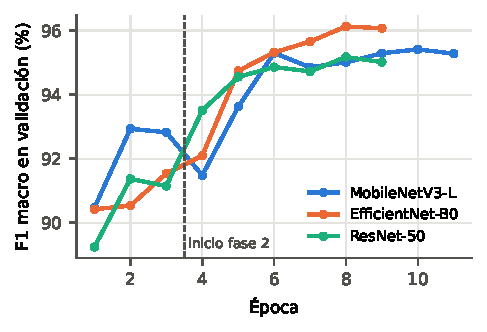
\includegraphics[width=\columnwidth]{figuras/fig_curvas.pdf}
\caption{F1 macro en validación por época. La línea discontinua marca el inicio de la fase~2 (ajuste de las últimas etapas).}
\label{fig:curvas}
\end{figure}

\subsection{Desempeño por clase del modelo seleccionado}
La Tabla~\ref{tab:clases} y la Fig.~\ref{fig:confusion} detallan el comportamiento de MobileNetV3. Papel/cartón y orgánico alcanzan los F1 más altos (\FPapMN\,\% y \FOrgMN\,\%), mientras que plástico, vidrio y metal quedan alrededor del 94\,\%. De los \errTotMN{} errores, los más frecuentes son vidrio confundido con metal (7), plástico con vidrio (5) y vidrio con plástico (4): materiales transparentes o reflectivos cuyo aspecto depende de la luz y del fondo más que de la textura. Este patrón contradice la hipótesis de la fase anterior, que anticipaba la mayor dificultad en la clase orgánica; en la práctica los restos de comida, con colores y formas irregulares, se separan con facilidad de los objetos manufacturados. La exactitud es de \accFuenteGcMN\,\% en las imágenes de Garbage Classification y de \accFuenteTnMN\,\% en las de TrashNet; el mismo patrón aparece en los otros dos modelos y probablemente se debe a que TrashNet concentra objetos transparentes o reflectivos fotografiados de cerca sobre fondo blanco, donde el contexto aporta poca información.

\begin{table}[t]
\caption{Precisión, exhaustividad y F1 por clase de MobileNetV3 en prueba (\%)}\label{tab:clases}
\centering\footnotesize
\begin{tabular}{@{}lrrrr@{}}
\toprule
Clase & $n$ & Precisión & Exhaustividad & F1 \\
\midrule
Plástico & \NPla & \PPlaMN & \RPlaMN & \FPlaMN \\
Papel/cartón & \NPap & \PPapMN & \RPapMN & \FPapMN \\
Vidrio & \NVid & \PVidMN & \RVidMN & \FVidMN \\
Metal & \NMet & \PMetMN & \RMetMN & \FMetMN \\
Orgánico & \NOrg & \POrgMN & \ROrgMN & \FOrgMN \\
\midrule
Macro & \nTest & & & \fMN \\
\bottomrule
\end{tabular}
\end{table}

\begin{figure}[t]
\centering
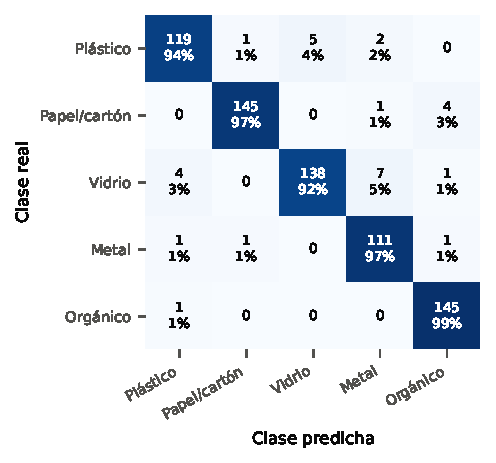
\includegraphics[width=0.92\columnwidth]{figuras/fig_confusion.pdf}
\caption{Matriz de confusión de MobileNetV3 en prueba (conteos y porcentaje por fila).}
\label{fig:confusion}
\end{figure}

\begin{figure*}[!t]
\centering
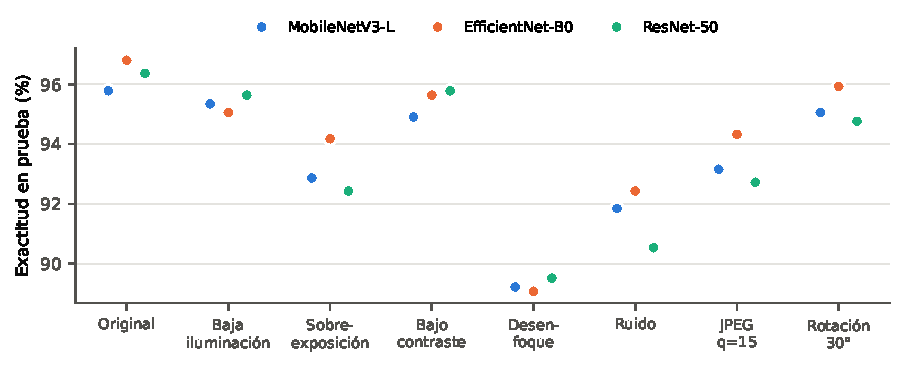
\includegraphics[width=0.9\textwidth]{figuras/fig_robustez.pdf}
\caption{Exactitud en prueba bajo perturbaciones de captura aplicadas a todas las imágenes.}
\label{fig:robustez}
\end{figure*}

\subsection{Calibración y rechazo de casos inciertos}
La temperatura ajustada en validación fue $T=\TMN$. Un valor menor que uno indica que el modelo era \emph{subconfiado}, un efecto esperado del suavizado de etiquetas \cite{szegedy2016}, que limita la probabilidad máxima durante el entrenamiento. Tras la calibración el ECE en prueba bajó de \eceRawMN\,\% a \eceCalMN\,\% y la log-verosimilitud negativa de \nllRawMN{} a \nllCalMN{} (Fig.~\ref{fig:fiabilidad}); antes de calibrar, las predicciones con confianza nominal entre 60 y 73\,\% acertaban más del 90\,\% de las veces y las de más de 80\,\% acertaban todas, de modo que un umbral sobre la confianza sin calibrar habría rechazado muchas predicciones correctas.

Con el umbral elegido en validación ($\tau=\umbralMN\,\%$), el agente decide automáticamente el \cobMN\,\% de las imágenes de prueba con una exactitud de \accSelMN\,\%, frente al \accMN\,\% de clasificar todo. De los \errTotMN{} errores, \errRevMN{} se envían a revisión manual en lugar de llegar al contenedor equivocado, a costa de revisar también \okRevMN{} aciertos. La Tabla~\ref{tab:operacion} muestra cómo exigir más precisión desplaza este equilibrio, y la Fig.~\ref{fig:riesgo} presenta la curva completa de riesgo y cobertura de los tres modelos. Con un objetivo del 99\,\%, MobileNetV3 deja pasar solo \opCErrMN{} errores a cambio de enviar a revisión \opCRevMN{} imágenes (cobertura de \opCCobMN\,\%). 

\begin{table}[t]
\caption{Puntos de operación de MobileNetV3 según la exactitud exigida en validación}\label{tab:operacion}
\centering\footnotesize\setlength{\tabcolsep}{4pt}
\begin{tabular}{@{}lrrrr@{}}
\toprule
Objetivo & $\tau$ (\%) & Cobertura (\%) & Exact. aceptadas (\%) & Errores autom. \\
\midrule
97\,\% & \opAUmbralMN & \opACobMN & \opASelMN & \opAErrMN \\
98\,\% & \opBUmbralMN & \opBCobMN & \opBSelMN & \opBErrMN \\
99\,\% & \opCUmbralMN & \opCCobMN & \opCSelMN & \opCErrMN \\
\midrule
Sin rechazo & -- & 100,0 & \accMN & \errTotMN \\
\bottomrule
\end{tabular}
\end{table}

\begin{figure}[t]
\centering
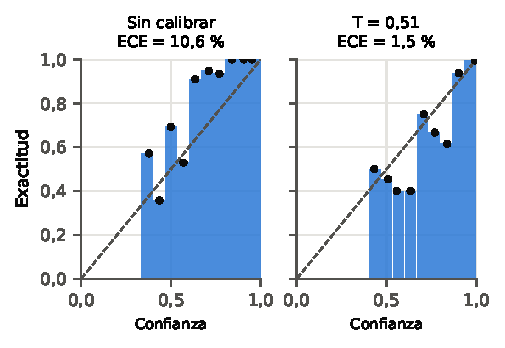
\includegraphics[width=\columnwidth]{figuras/fig_fiabilidad.pdf}
\caption{Diagramas de fiabilidad de MobileNetV3 en prueba antes y después del escalamiento de temperatura. La diagonal representa una calibración perfecta.}
\label{fig:fiabilidad}
\end{figure}

\begin{figure}[t]
\centering
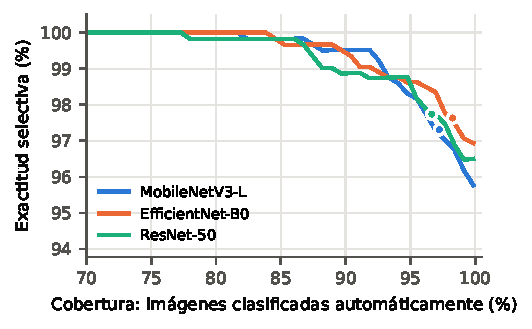
\includegraphics[width=\columnwidth]{figuras/fig_riesgo_cobertura.pdf}
\caption{Exactitud de las decisiones automáticas en función de la cobertura. Los puntos marcan el umbral elegido en validación para cada modelo.}
\label{fig:riesgo}
\end{figure}

\begin{figure*}[!t]
\centering
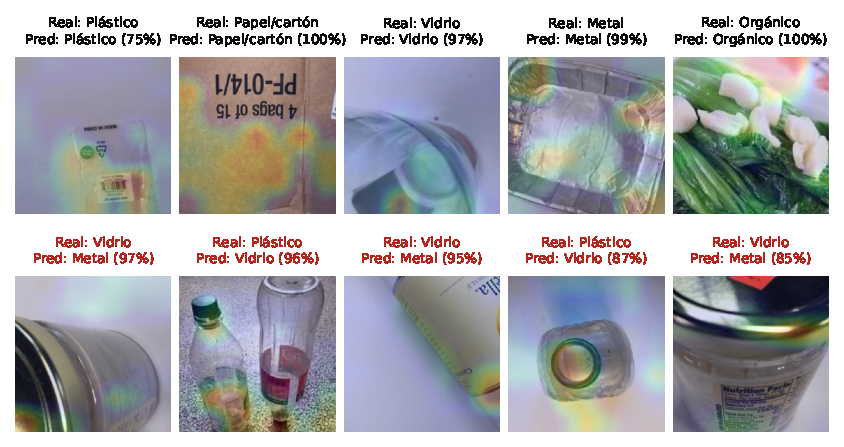
\includegraphics[width=0.9\textwidth]{figuras/fig_gradcam.pdf}
\caption{Mapas Grad-CAM de MobileNetV3 sobre imágenes de prueba. Fila superior: un acierto por clase. Fila inferior: los cinco errores con mayor confianza (título en rojo).}
\label{fig:gradcam}
\end{figure*}

\begin{figure}[!t]
\centering
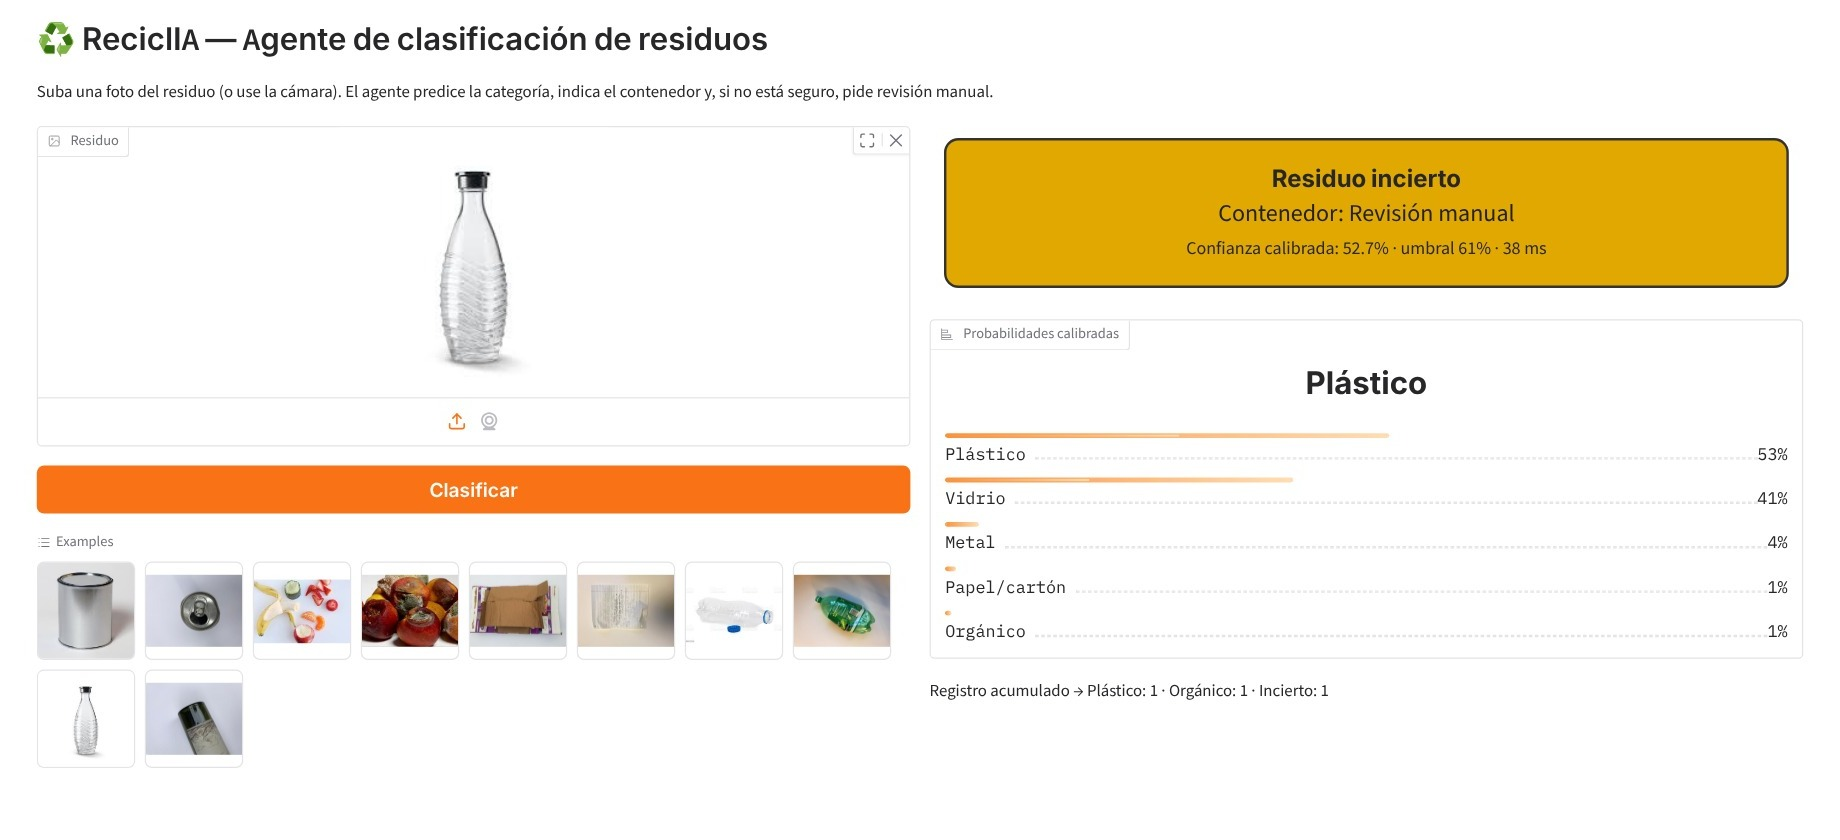
\includegraphics[width=\columnwidth]{figuras/fig_demo.jpg}
\caption{Demostración web del agente. Una botella de vidrio con forma de botella plástica produce una predicción dividida entre plástico y vidrio, y el agente la marca como residuo incierto.}
\label{fig:demo}
\end{figure}

\subsection{Robustez ante condiciones de captura}
La Fig.~\ref{fig:robustez} resume la exactitud de los tres modelos bajo las siete perturbaciones. Para MobileNetV3, la baja iluminación (\robOscuroMN\,\%), el bajo contraste (\robContrasteMN\,\%) y la rotación (\robRotMN\,\%) apenas afectan el desempeño, gracias al aumento de datos fotométrico y geométrico. Las caídas más fuertes se dan con desenfoque (\robBlurMN\,\%), ruido (\robRuidoMN\,\%) y sobreexposición (\robClaroMN\,\%), condiciones que borran la textura o los reflejos que distinguen vidrio, plástico y metal. El mecanismo de rechazo reacciona a la degradación: la tasa de revisión manual pasa de \robRechOrigMN\,\% en las imágenes originales a \robRechBlurMN\,\% con desenfoque y \robRechRuidoMN\,\% con ruido, aunque no alcanza a compensar toda la pérdida (exactitud sobre aceptadas de \robSelBlurMN\,\% con desenfoque). Esto indica que la cámara de la estación debe tener enfoque fijo y una iluminación estable.


\subsection{Interpretabilidad}
La Fig.~\ref{fig:gradcam} muestra mapas Grad-CAM de MobileNetV3. En los aciertos la activación cae principalmente sobre el objeto (la superficie del cartón, la bandeja metálica, los restos de comida) y no sobre el fondo, lo que sugiere que el modelo no depende solo del estilo fotográfico de cada fuente. En los errores de mayor confianza, todos entre vidrio, plástico y metal, la activación se concentra en bordes, tapas y bandas brillantes del recipiente: zonas donde los tres materiales se parecen, coherente con las confusiones de la Fig.~\ref{fig:confusion}.


\subsection{Latencia y demostración}
En un solo hilo de CPU, MobileNetV3 tarda \latUnoMN~ms por imagen (percentil 95: \latUnoPnMN~ms), a lo que se suman unos \latPreMN~ms de lectura y preprocesamiento. El ciclo completo queda muy por debajo de la meta de 300~ms fijada en la fase anterior, lo que permite operar en tiempo real incluso en equipos modestos. La Fig.~\ref{fig:demo} muestra la demostración web: el agente presenta la categoría, el contenedor, la confianza calibrada y el acumulado del registro; ante una botella de vidrio con forma típica de botella plástica, la confianza (53\,\%) queda bajo el umbral y el agente solicita revisión manual.


\subsection{Limitaciones}\label{sec:discusion}
Los resultados deben leerse con tres cautelas. Primero, todas las imágenes de orgánicos provienen de Garbage Classification, de modo que parte de la facilidad de esa clase puede deberse al estilo de las fotografías de esa fuente y no solo al material; Grad-CAM sugiere que el modelo atiende al objeto, pero la prueba definitiva es evaluar con fotografías propias de la estación. Segundo, las perturbaciones son sintéticas y no reproducen sombras, oclusiones ni varios objetos en escena. Tercero, la latencia se midió en un servidor y no en el dispositivo de borde final, aunque la diferencia de órdenes de magnitud con la meta de 300~ms deja un margen amplio.

% =====================================================================
\section{Conclusiones}\label{sec:conclusiones}
% =====================================================================
Este trabajo convirtió la propuesta de las fases anteriores en un agente funcional para clasificar residuos en el punto de depósito. Tres resultados resumen el aporte. Primero, combinar fuentes públicas exige deduplicar: casi todo TrashNet está contenido en Garbage Classification y, sin depurar, las mismas fotografías habrían quedado en entrenamiento y en prueba. Segundo, MobileNetV3-Large alcanza \accMN\,\% de exactitud y \fMN\,\% de F1 macro con \latUnoMN~ms por imagen en un núcleo de CPU; EfficientNet-B0 obtiene una cifra algo mayor sin diferencia estadísticamente significativa (McNemar, $p=\mcnMNEF$) y con mayor latencia, por lo que MobileNetV3 es la opción preferida para el despliegue. Tercero, calibrar la confianza permite que el agente se abstenga con criterio: con el umbral elegido decide el \cobMN\,\% de los casos con \accSelMN\,\% de exactitud y desvía a revisión manual \errRevMN{} de los \errTotMN{} errores, y el umbral puede ajustarse según cuánto error tolere la estación.

Como trabajo futuro se proponen: capturar un conjunto propio de imágenes en la estación de la universidad, con orgánicos y fondos reales, para validar la generalización; desplegar el modelo cuantizado en un dispositivo de bajo costo y medir allí la latencia; extender el agente a detección de varios objetos por imagen, y conectar la decisión a un actuador físico que dirija el residuo al contenedor.

\section*{Disponibilidad de código, datos y video}
Código fuente, modelo entrenado e instrucciones: \linkGithub. Conjunto de datos procesado (\nTotal{} imágenes, particiones y manifiesto): \linkDrive. Video promocional de la aplicación: \linkVideo.

\balance
\bibliographystyle{ieeetr}
\bibliography{referencias}

\end{document}
